\documentclass{article}
%packages
\usepackage{graphicx}
\usepackage[utf8]{inputenc}
\usepackage[T1]{fontenc}
\usepackage[frenchb]{babel}
\usepackage[a4paper]{geometry}

\begin{document}
%title
\begin{titlepage}
	\vspace{-20px}
	\begin{tabular}{l}
		\textsc{Blin} S\'ebastien\\
		\textsc{Collin} Pierre-Henri
	\end{tabular}
	\hfill \vspace{10px}
\includegraphics[scale=0.1]{esir.png}\\
	\vfill
	\begin{center}
		\Huge{\'Ecole sup\'erieure d'ing\'enieurs de Rennes}\\
		\vspace{1cm}
		\LARGE{1\`ere Ann\'ee}\\
		\large{Parcours Informatique}\\
		\vspace{0.5cm}\hrule\vspace{0.5cm}
		\LARGE{\textbf{Algorithmie et complexité}}\\
		\Large{Compte-Rendu TP1}
		\vspace{0.5cm}\hrule
		\vfill
		\vfill
	\end{center}
	\begin{flushleft}
		\Large{Sous l'encadrement de~:}\\
		\vspace{0.2cm}
		\large{{Ridoux} Olivier}\\
		\large{{Maurel} Pierre}
	\end{flushleft}
	\vfill
\end{titlepage}

\section{Objectif}
Ce premier TP d'Algorithmie et Complexité a pour objectif de comparer 2 algorithmes de tri de 2 complexités différentes. Le premier (tri par insertion) a en effet une complexité théorique en $O(n^2)$, contre $O(nlogn)$ pour le second tri étudié (tri fusion). La dernière partie du TP consistait à examiner un programme et à regarder sa complexité.
\section{Moyens mis en \oe uvre}
Pour réaliser ce TP, nous avions à disposition un fichier JAVA à compléter qui s'occupait de l'implementation des tris ainsi que la mesure du temps de calcul. Puis un programme Matlab pour l'affichage des graphes de résultats.\\
Voici notre implémentation du tri insertion :\\
\begin{verbatim}
public static void triInsertion(int[] t){
    for (int i = 1; i < t.length; i++) {
      int valueToSort = t[i];
      int j = 0;
      for(j = i; j > 0 && t[j - 1] > valueToSort; --j) {
        t[j] = t[j - 1];
      }
      t[j] = valueToSort;
    }
  }
\end{verbatim}
Et le tri fusion :
\begin{verbatim}
/* Sous-fonction (recursive) pour le tri fusion
   * Trie le sous-tableau t[debut]..t[fin]
   */
private static void triFusion(int[] t, int debut, int fin){
  if(debut < fin)
  {
    int milieu = (debut+fin)/2;
    triFusion(t, debut, milieu);
    triFusion(t, milieu+1, fin);
    fusionner(t, debut, milieu, fin);
  }
}
\end{verbatim}
\section{Résultats}
Pour le tri insertion, pour trier 60 000 000 de résultats il faut :
\begin{itemize}
  \item 33 ms dans le meilleur cas (croissant)
  \item 380 minutes dans un cas normal
  \item 12 jours dans le pire des cas
\end{itemize}
Avec les courbes correspondantes :
\begin{figure}
	\begin{center}
		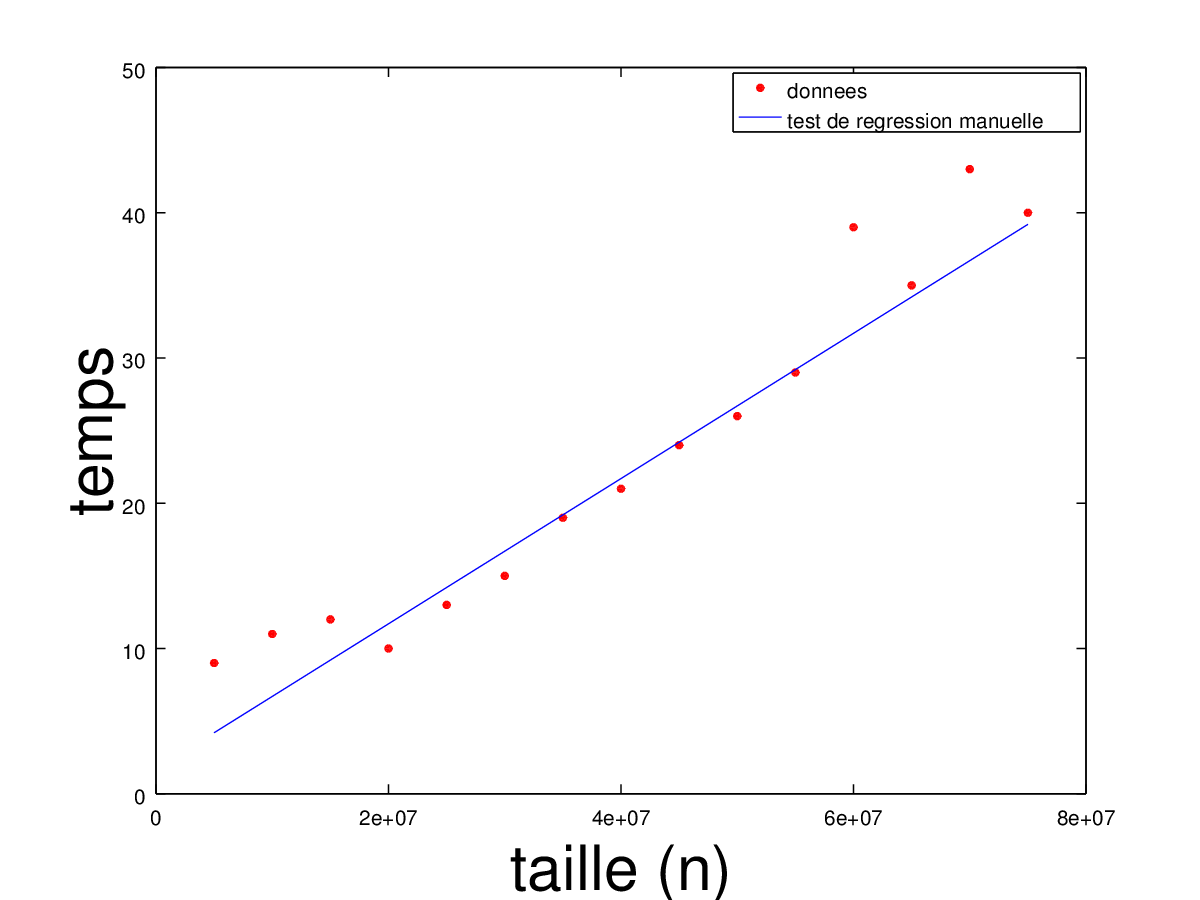
\includegraphics[scale=0.7]{croissant}\\
		Tri insertion cas croissant
	\end{center}
\end{figure}
\begin{figure}
	\begin{center}
		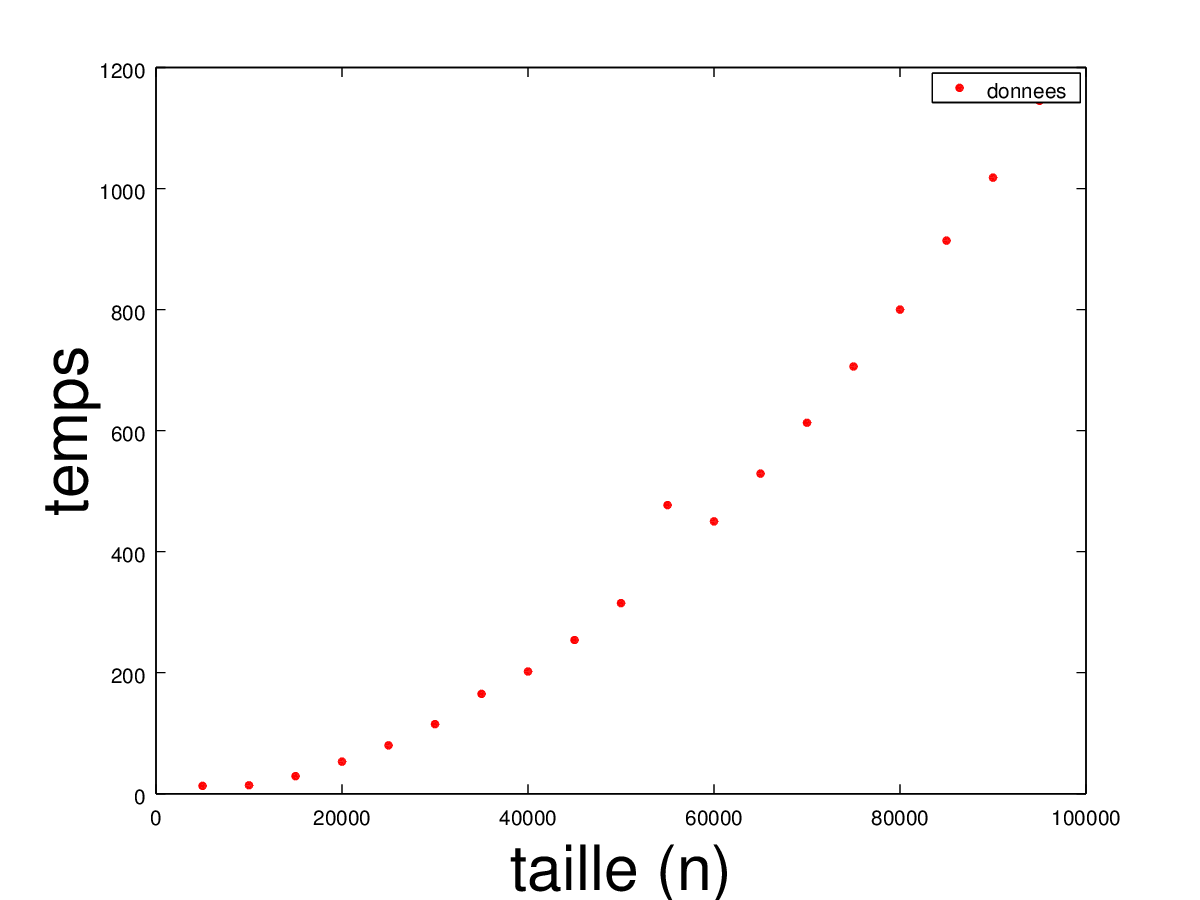
\includegraphics[scale=0.7]{random}\\
		Tri insertion cas aléatoire
	\end{center}
\end{figure}
\begin{figure}
	\begin{center}
		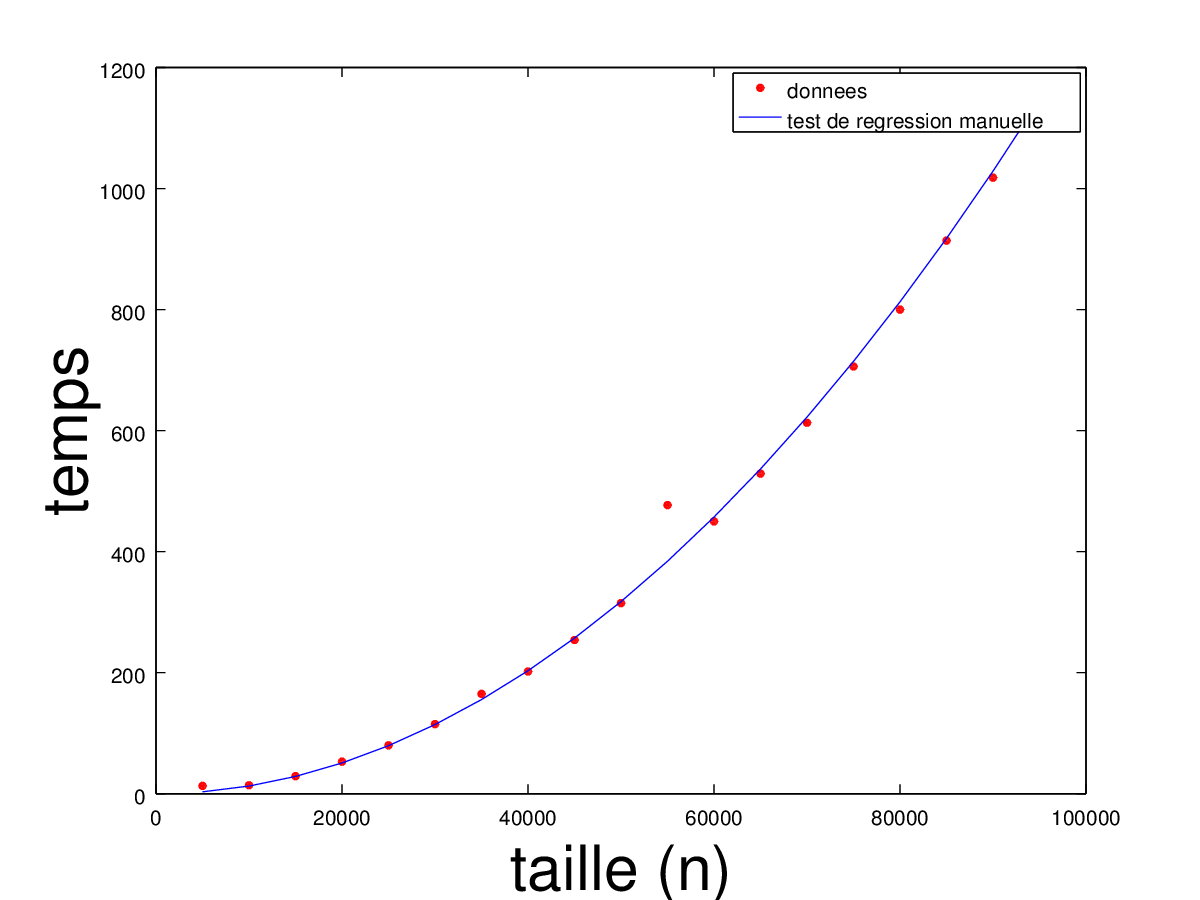
\includegraphics[scale=0.7]{decroissant}\\
		Tri insertion cas décroissant
	\end{center}
\end{figure}
On obtient une complexité en $O(n^2)$\\
Pour le tri fusion, on obtient un temps < 10 secondes :
\begin{figure}
	\begin{center}
		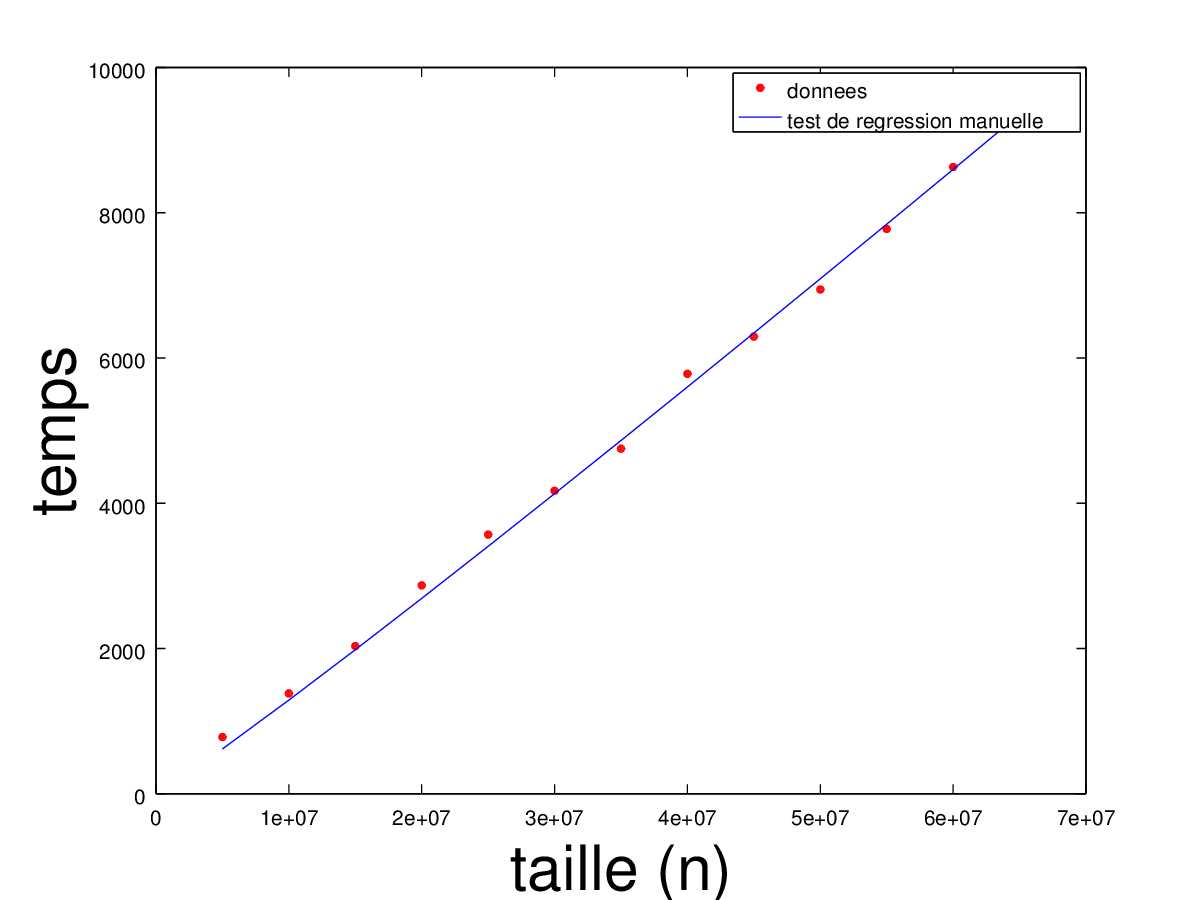
\includegraphics[scale=0.7]{fusion}\\
		Tri fusion
	\end{center}
\end{figure}
L'analyse de l'algorithme de permutation (qui cherche toutes les combinaisons avec les n premières lettres de l'alphabet) de la partie 3 nous a donné une complexité factorielle. On remarque qu'elle est très difficile à tracer et que son temps est très vite insupportable.
\section{Conclusion}
Dans ce TP, nous avons donc pu découvrir et implémenter 3 algorithmes de complexité différentes. Nous pouvons en conclure que $O(n!) >>>> O(n^2) >>>> O(nlogn) > O(n)$

\end{document}

